\begin{figure}[t!]
\centering
\tikzstyle{every node}=[scale=0.88]
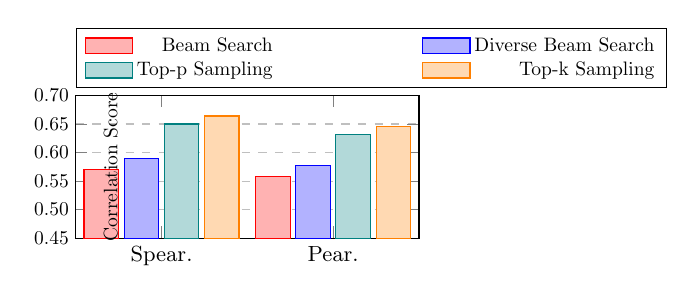
\begin{tikzpicture}
    \begin{axis}[
      ymajorgrids,
      grid style=dashed,
      legend style={at={(0,1.05)}, anchor=south west, nodes={scale=0.8},/tikz/every even column/.append style={column sep=1.85cm}},
      legend cell align={right},
      legend columns=2,
      ybar,
      enlarge x limits=0.5,
      xtick align=inside,
      height=.28\textwidth,
      width=.49\textwidth,
      bar width=0.8em,
      ylabel={Correlation Score},
      symbolic x coords={{1}, {2}},
      xtick=data,
      nodes near coords align={vertical},
      xticklabels={\small Spear., \small Pear.},
      ymin=0.45, ymax=0.70,
      ytick={0.45,0.50,...,0.70},
      legend entries={Beam Search,Diverse Beam Search,Top-p Sampling,Top-k Sampling},
      ylabel style={at={(-0.1,0.5)}, yshift=-3.4em, scale=0.8},xlabel style={yshift=0.3em,align=center},
      y tick label style={scale=0.8,
                        /pgf/number format/fixed,
                        /pgf/number format/fixed zerofill,
                        /pgf/number format/precision=2},
      bar width=1.25em,
      % nodes near coords,
      % every node near coord/.append style={
      % font=\scriptsize,
      % /pgf/number format/fixed,
      % /pgf/number format/fixed zerofill,
      % /pgf/number format/precision=3,
      % xshift=-0.1em},
      ]
      \addplot[fill=red!30, draw=red,area legend] coordinates {({1},0.570) ({2},0.558) };

      \addplot[fill=blue!30, draw=blue,area legend] coordinates {({1},0.589) ({2},0.577) };

      \addplot[fill=teal!30, draw=teal,area legend] coordinates {({1},0.650) ({2},0.631) };

      \addplot[fill=orange!30, draw=orange,area legend] coordinates {({1},0.664) ({2},0.645) };

    \end{axis}
    \end{tikzpicture}
    \vspace{-3mm}
    \caption{
    Correlation scores of the evaluation models learned by CSEM and ChatGPT on the multi-aspect evaluation.
    }
    \label{fig_diff_sampling_methods}
\end{figure}